\chapter{Atlas cualitativo del corpus externo}
\label{app:external-case-atlas}

Este anexo presenta visualmente los doce casos externos fijados antes de abrir las salidas. Cada
comparación conserva la página completa y alinea referencia HR, entrada LR ampliada por vecino más
próximo, EDSR oficial y EDSR adaptado. Los casos \texttt{three-revelations} y
\texttt{mari-carmen} se muestran en el capítulo de resultados
(Figuras~\ref{fig:external-accepted} y~\ref{fig:external-rejected}); las diez láminas restantes se
incluyen a continuación. De este modo, ninguna decisión cualitativa queda respaldada únicamente por
un recuento o por una selección favorable de imágenes.

La Tabla~\ref{tab:external-atlas-index} actúa como índice y conserva para cada caso la decisión y el
origen observable del daño. \emph{No recuperado} indica que la limitación ya estaba presente en LR;
\emph{sin defecto nuevo claro} no afirma perfección, sino que el revisor no identificó un daño nuevo
atribuible al EDSR adaptado. Las doce valoraciones proceden de un único revisor no ciego y no deben
interpretarse como tasas poblacionales.

\begin{table}[htbp]
  \centering
  \scriptsize
  \setlength{\tabcolsep}{2.5pt}
  \caption{Índice de los doce casos externos completos. Fuente: elaboración propia a partir de la
  revisión cualitativa fija.}
  \label{tab:external-atlas-index}
  \begin{tabular}{p{0.25\textwidth}p{0.13\textwidth}p{0.22\textwidth}p{0.25\textwidth}}
    \toprule
    Obra y condición & Decisión & Origen del daño & Localización \\
    \midrule
    \emph{Cullera Suite}; x2 limpia & Aceptable & Sin defecto nuevo claro & Fig.~\ref{fig:external-cullera} \\
    \emph{El jardín de Hera}; x2 limpia & Aceptable & Sin defecto nuevo claro & Fig.~\ref{fig:external-hera} \\
    \emph{How to Train Your Dragon}; x2 moderada & Aceptable & Sin defecto nuevo claro & Fig.~\ref{fig:external-dragon} \\
    \emph{Xàtiva 1939}; x2 moderada & Aceptable & Sin defecto nuevo claro & Fig.~\ref{fig:external-xativa} \\
    \emph{Malaguenya de Barxeta}; x2 fuerte & Aceptable & No recuperado de LR & Fig.~\ref{fig:external-malaguenya} \\
    \emph{Three Revelations}; x2 fuerte & Aceptable & No recuperado de LR & Fig.~\ref{fig:external-accepted} \\
    \emph{Capitania Cides}; x4 limpia & Aceptable & Sin defecto nuevo claro & Fig.~\ref{fig:external-capitania} \\
    \emph{La rosa i el drac}; x4 limpia & Con reservas & No recuperado de LR & Fig.~\ref{fig:external-rosa} \\
    \emph{City in Three Words}; x4 moderada & Con reservas & No recuperado de LR & Fig.~\ref{fig:external-city} \\
    \emph{Lorencín Mendoza}; x4 moderada & Aceptable & No recuperado de LR & Fig.~\ref{fig:external-lorencin} \\
    \emph{Theme from Jurassic Park}; x4 fuerte & Con reservas & No recuperado de LR & Fig.~\ref{fig:external-jurassic} \\
    \emph{Mari Carmen}; x4 fuerte & Rechazado & No recuperado de LR & Fig.~\ref{fig:external-rejected} \\
    \bottomrule
  \end{tabular}
\end{table}

\begin{figure}[p]
  \centering
  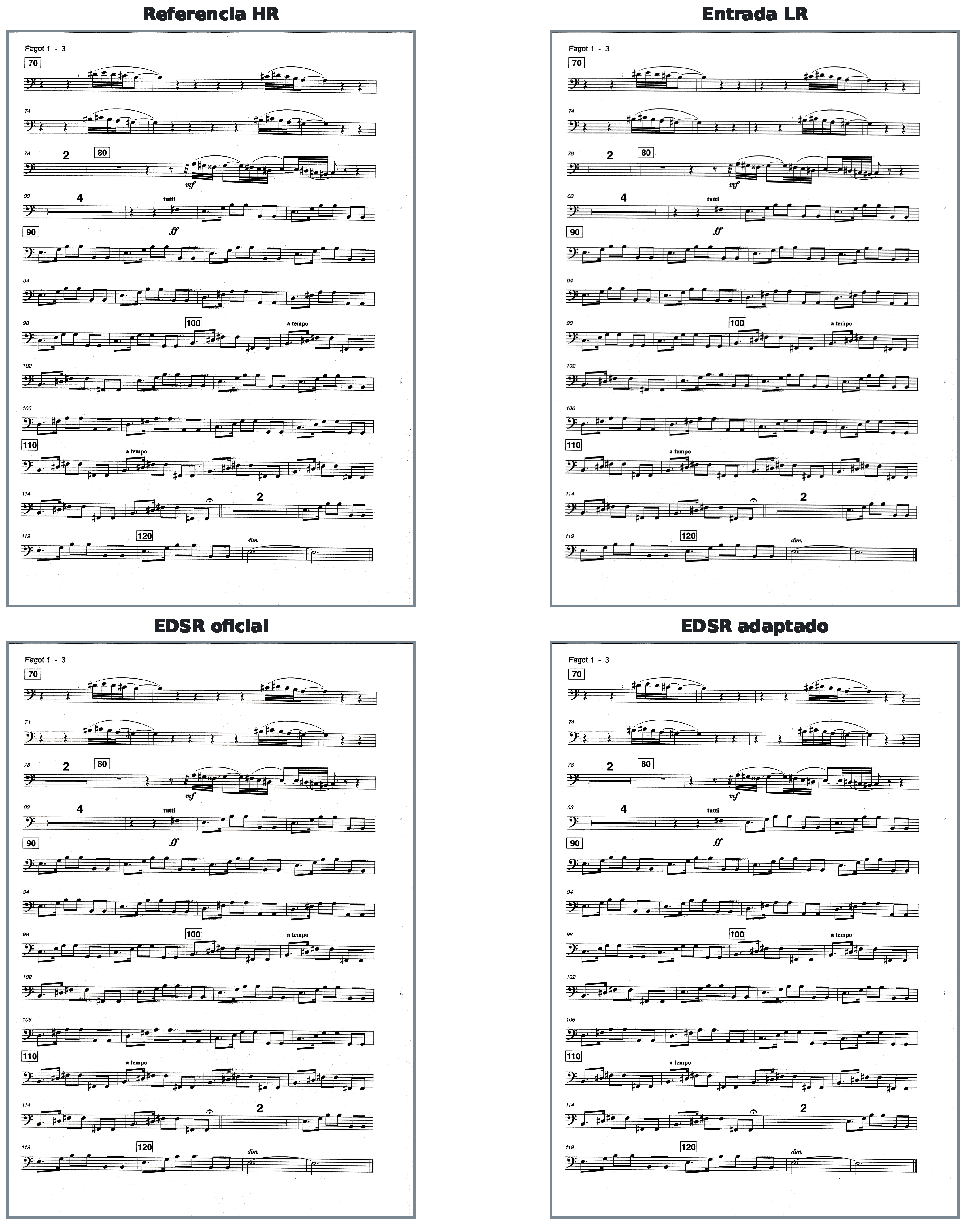
\includegraphics[width=\textwidth,height=0.80\textheight,keepaspectratio]{figures/results/external-cullera-suite-full-page-x2-clean.pdf}
  \caption[Corpus externo: Cullera Suite, x2 limpia]{Caso fijo \texttt{cullera-suite}, x2 limpia,
  aceptado sin defecto nuevo claro. La adaptación aporta una mejora sutil de definición sin alterar
  la estructura global. Parte de fagot primero de \emph{Cullera Suite}, de Rafael Talens. Fuente:
  archivo musical de la SJMA; página reproducida con autorización expresa para este TFG. LR y
  reconstrucciones son transformaciones de elaboración propia.}
  \label{fig:external-cullera}
\end{figure}
\clearpage

\begin{figure}[p]
  \centering
  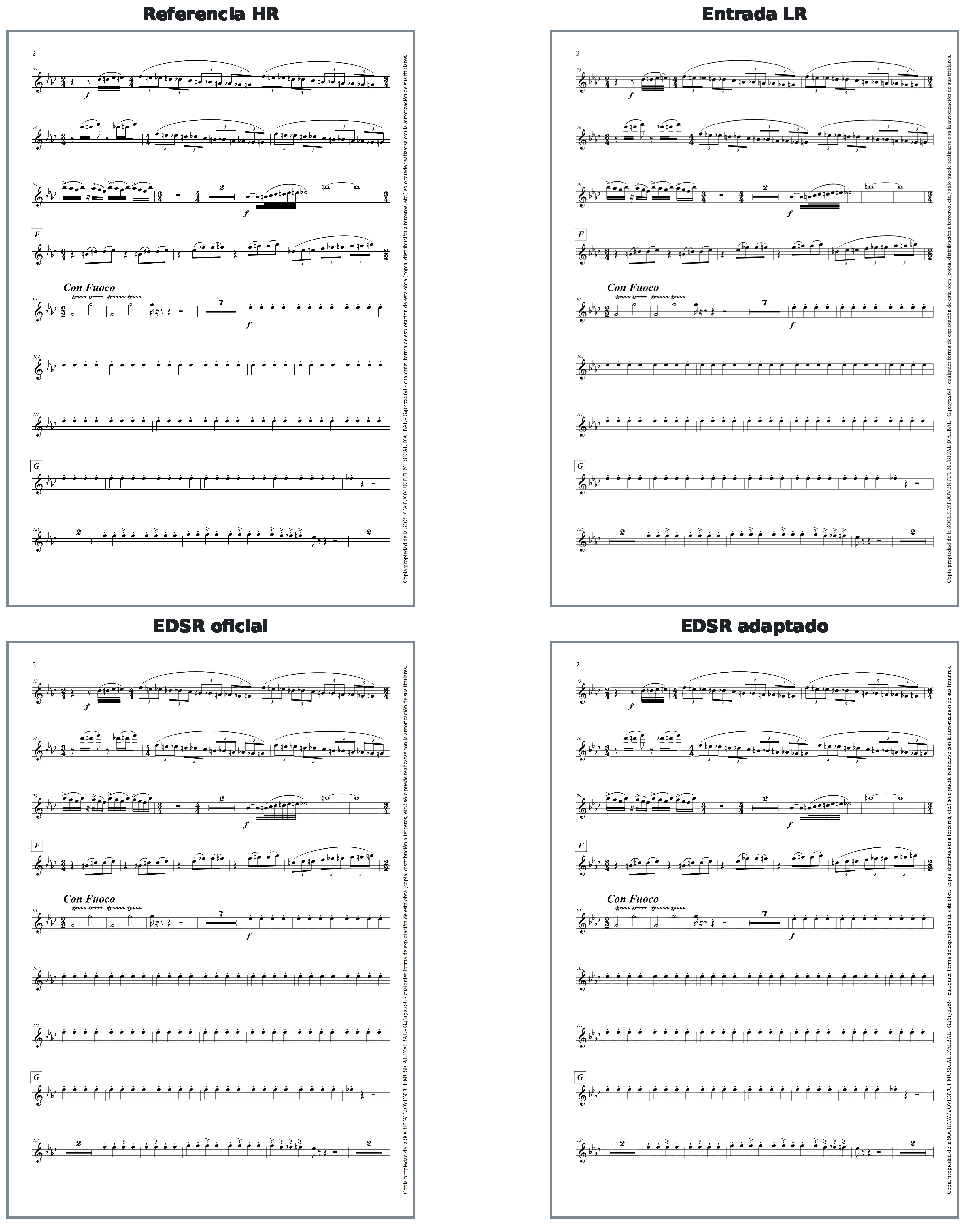
\includegraphics[width=\textwidth,height=0.80\textheight,keepaspectratio]{figures/results/external-el-jardin-de-hera-full-page-x2-clean.pdf}
  \caption[Corpus externo: El jardín de Hera, x2 limpia]{Caso fijo
  \texttt{el-jardin-de-hera}, x2 limpia, aceptado sin defecto nuevo claro. El EDSR adaptado conserva
  la página y ofrece más claridad que el oficial. Parte de oboe primero de \emph{El jardín de Hera},
  de José Suñer. Fuente: archivo musical de la SJMA; página reproducida con autorización expresa
  para este TFG. LR y reconstrucciones son transformaciones de elaboración propia.}
  \label{fig:external-hera}
\end{figure}
\clearpage

\begin{figure}[p]
  \centering
  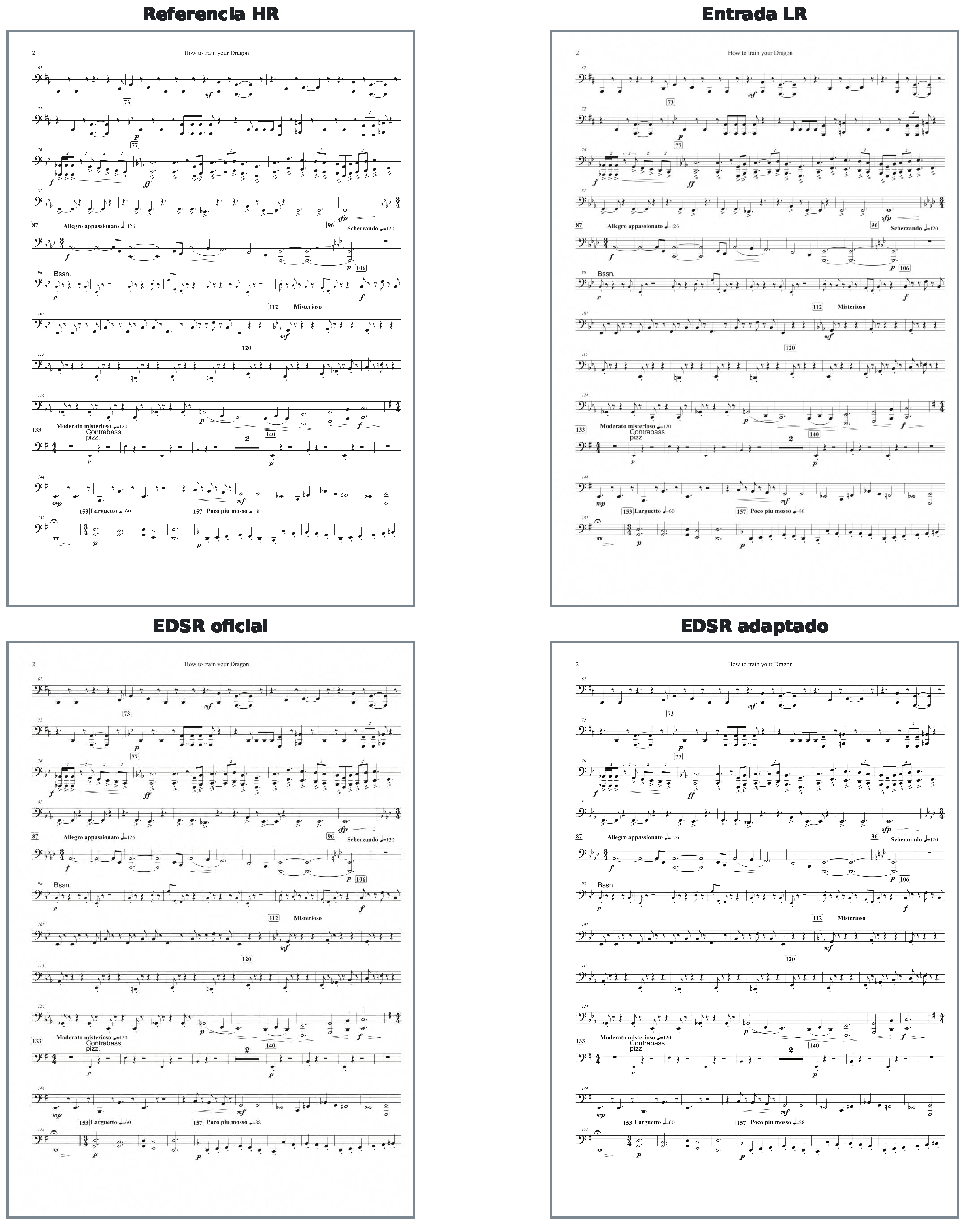
\includegraphics[width=\textwidth,height=0.80\textheight,keepaspectratio]{figures/results/external-how-to-train-your-dragon-full-page-x2-moderate.pdf}
  \caption[Corpus externo: How to Train Your Dragon, x2 moderada]{Caso fijo
  \texttt{how-to-train-your-dragon}, x2 moderada, aceptado sin defecto nuevo claro. La adaptación
  reduce el desenfoque y los halos del EDSR oficial. Parte de tuba de \emph{How to Train Your
  Dragon}, música de John Powell. Fuente: archivo musical de la SJMA; página reproducida con
  autorización expresa para este TFG. LR y reconstrucciones son transformaciones de elaboración
  propia.}
  \label{fig:external-dragon}
\end{figure}
\clearpage

\begin{figure}[p]
  \centering
  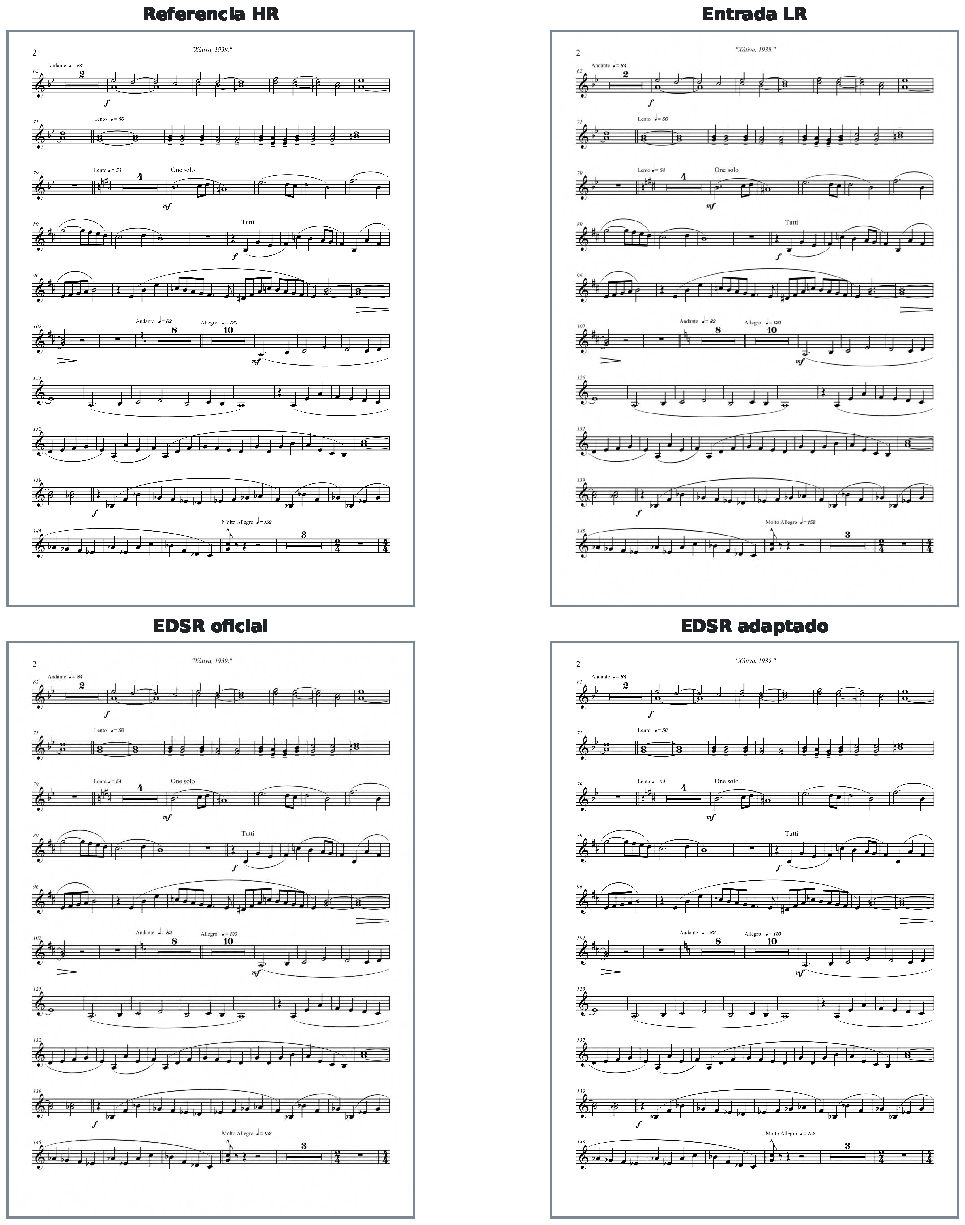
\includegraphics[width=\textwidth,height=0.80\textheight,keepaspectratio]{figures/results/external-xativa-1939-full-page-x2-moderate.pdf}
  \caption[Corpus externo: Xàtiva 1939, x2 moderada]{Caso fijo \texttt{xativa-1939}, x2 moderada,
  aceptado sin defecto nuevo claro. El EDSR adaptado define mejor la notación que el oficial; el
  texto sigue siendo el elemento más sensible. Parte de trompas primera y segunda de \emph{Xàtiva
  1939: El Guernica valencià}, de David Penadés-Fasanar. Fuente: archivo musical de la SJMA; página
  reproducida con autorización expresa para este TFG. LR y reconstrucciones son transformaciones
  de elaboración propia.}
  \label{fig:external-xativa}
\end{figure}
\clearpage

\begin{figure}[p]
  \centering
  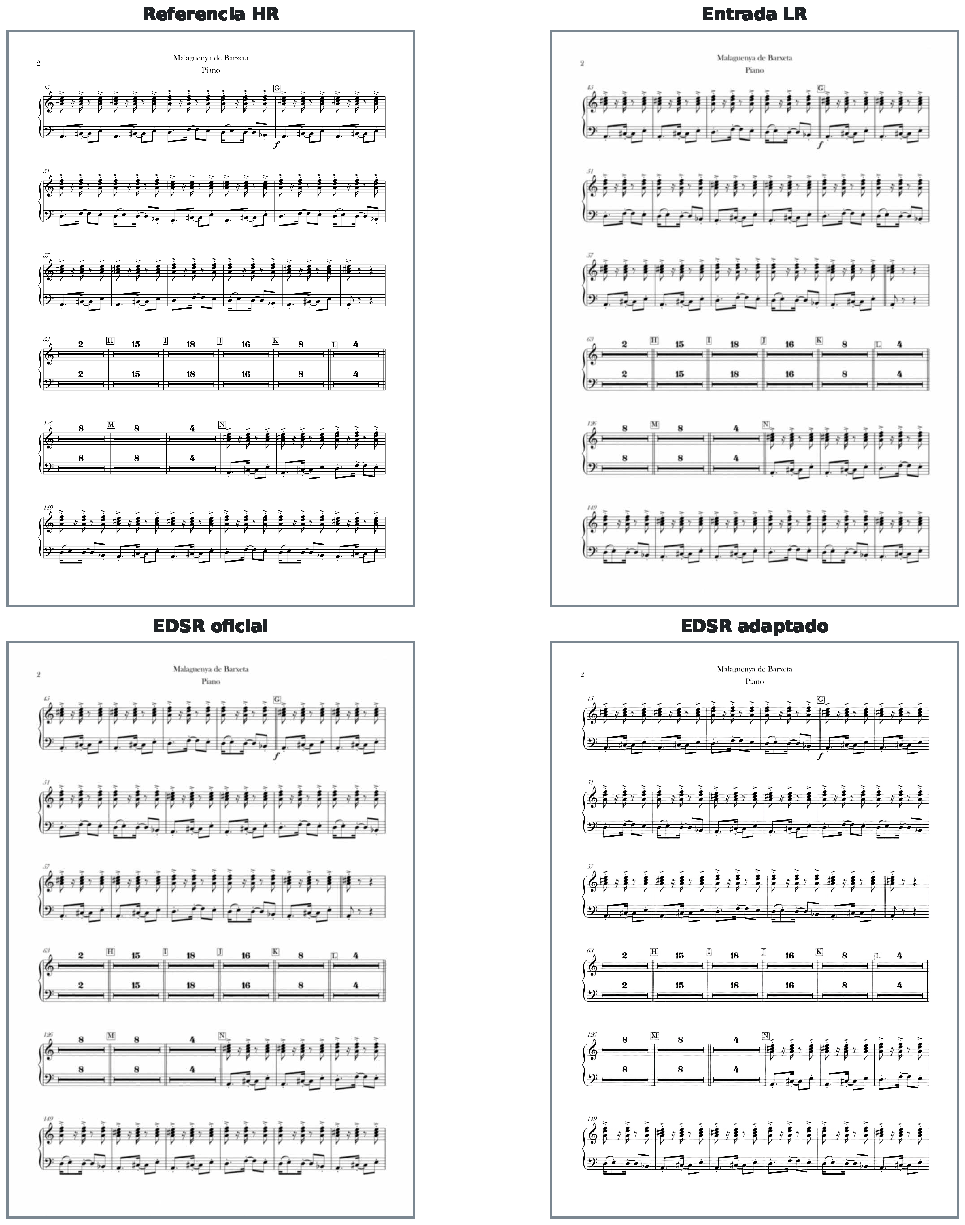
\includegraphics[width=\textwidth,height=0.80\textheight,keepaspectratio]{figures/results/external-malaguenya-de-barxeta-full-page-x2-strong.pdf}
  \caption[Corpus externo: Malaguenya de Barxeta, x2 fuerte]{Caso fijo
  \texttt{malaguenya-de-barxeta}, x2 fuerte, aceptado para consulta con daño de LR no recuperado. La
  adaptación mejora claramente al EDSR oficial y mantiene legible la notación principal, pero no
  restituye el texto y los dígitos pequeños. Parte de piano de \emph{Malaguenya de Barxeta}, de
  Azael Tormo. Fuente: archivo musical de la SJMA; página reproducida con autorización expresa para
  este TFG. LR y reconstrucciones son transformaciones de elaboración propia.}
  \label{fig:external-malaguenya}
\end{figure}
\clearpage

\begin{figure}[p]
  \centering
  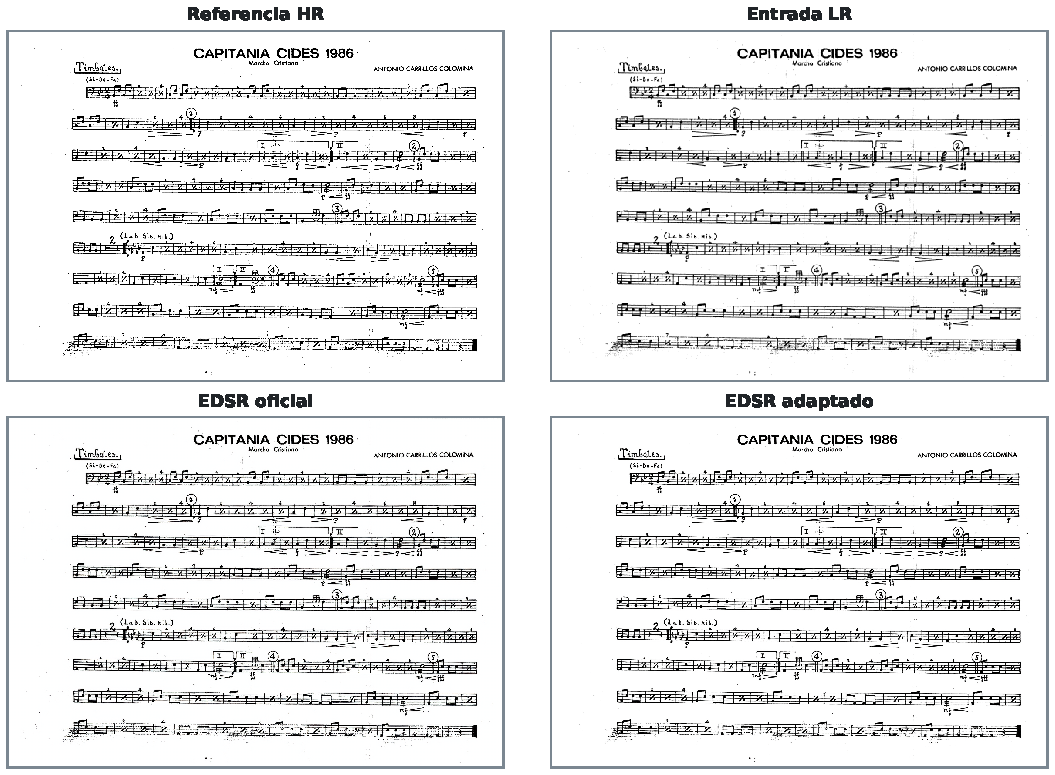
\includegraphics[width=\textwidth,height=0.80\textheight,keepaspectratio]{figures/results/external-capitania-cides-full-page-x4-clean.pdf}
  \caption[Corpus externo: Capitania Cides, x4 limpia]{Caso fijo \texttt{capitania-cides}, x4
  limpia, aceptado sin defecto nuevo claro. Sobre esta fuente escaneada, el adaptado limpia trazos
  sin desplazar la condición documental de HR como referencia. Parte de percusión y timbales de
  \emph{Capitania Cides}, de Antonio Carrillos. Fuente: archivo musical de la SJMA; página
  reproducida con autorización expresa para este TFG. LR y reconstrucciones son transformaciones
  de elaboración propia.}
  \label{fig:external-capitania}
\end{figure}
\clearpage

\begin{figure}[p]
  \centering
  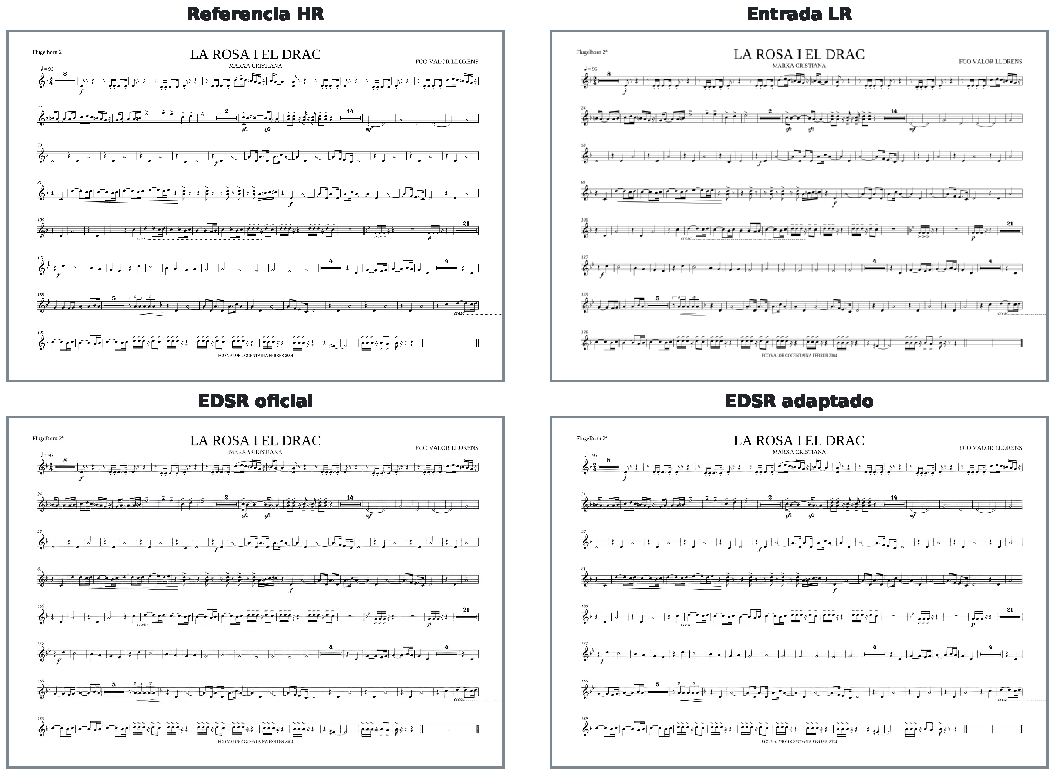
\includegraphics[width=\textwidth,height=0.80\textheight,keepaspectratio]{figures/results/external-la-rosa-i-el-drac-full-page-x4-clean.pdf}
  \caption[Corpus externo: La rosa i el drac, x4 limpia]{Caso fijo \texttt{la-rosa-i-el-drac}, x4
  limpia, aceptado con reservas por daño de LR no recuperado. El adaptado elimina parte del halo del
  EDSR oficial, pero el texto no recupera su legibilidad. Parte de fliscorno segundo de \emph{La
  rosa i el drac}, de Francisco Valor. Fuente: archivo musical de la SJMA; página reproducida con
  autorización expresa para este TFG. LR y reconstrucciones son transformaciones de elaboración
  propia.}
  \label{fig:external-rosa}
\end{figure}
\clearpage

\begin{figure}[p]
  \centering
  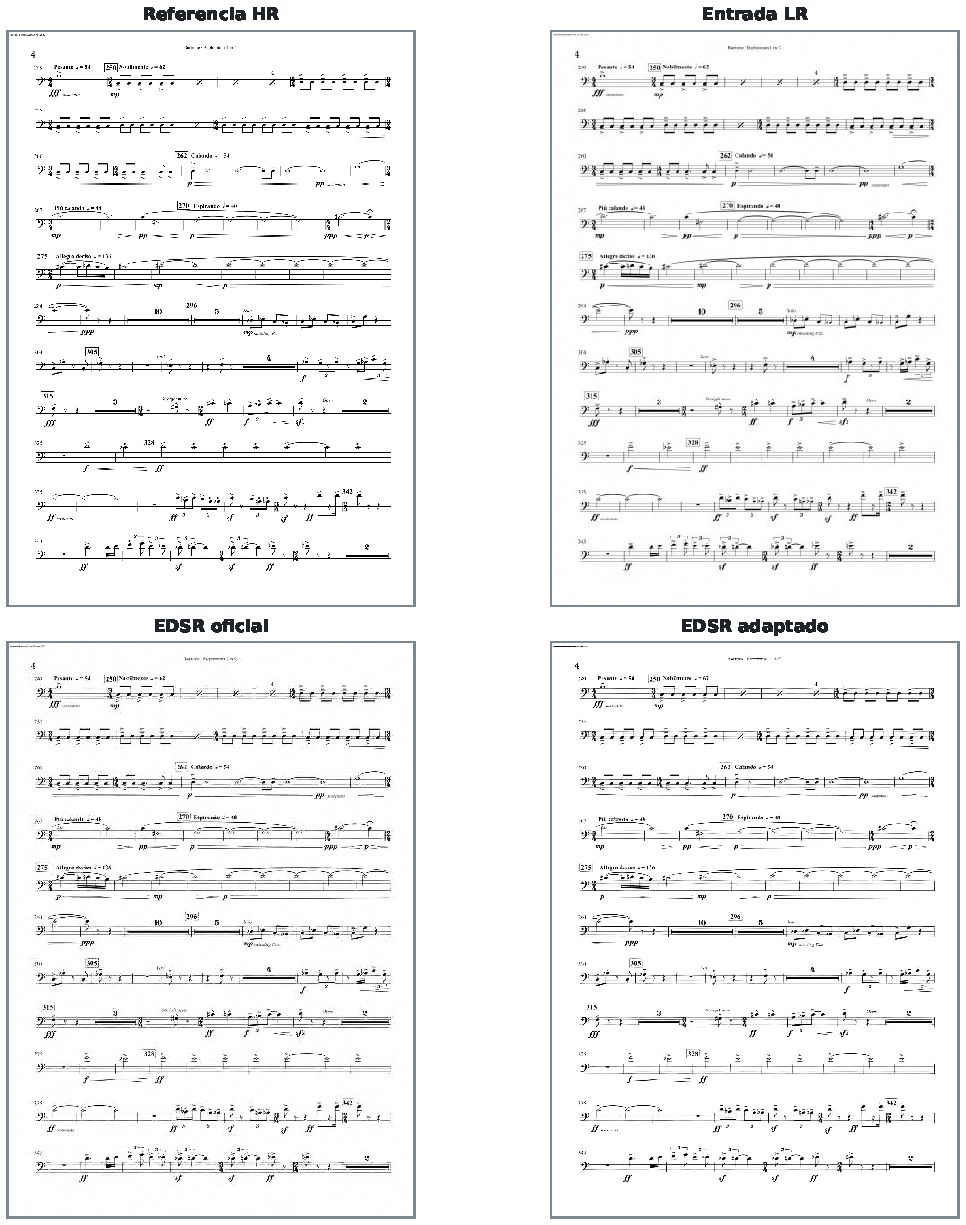
\includegraphics[width=\textwidth,height=0.80\textheight,keepaspectratio]{figures/results/external-city-in-three-words-full-page-x4-moderate.pdf}
  \caption[Corpus externo: City in Three Words, x4 moderada]{Caso fijo
  \texttt{city-in-three-words}, x4 moderada, aceptado con reservas por daño de LR no recuperado. La
  adaptación produce una página más limpia que el EDSR oficial, aunque la información textual fina
  sigue degradada. Parte de bombardino primero de \emph{City in Three Words}, de Carlos Pellicer.
  Fuente: archivo musical de la SJMA; página reproducida con autorización expresa para este TFG. LR
  y reconstrucciones son transformaciones de elaboración propia.}
  \label{fig:external-city}
\end{figure}
\clearpage

\begin{figure}[p]
  \centering
  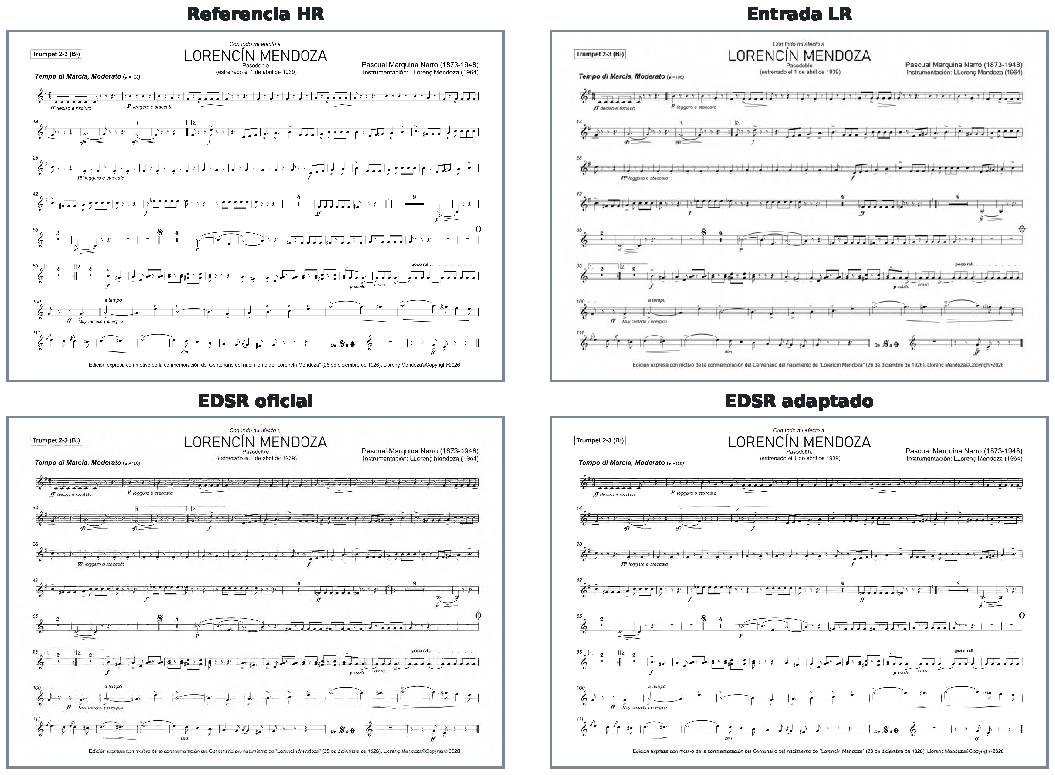
\includegraphics[width=\textwidth,height=0.80\textheight,keepaspectratio]{figures/results/external-lorencin-mendoza-full-page-x4-moderate.pdf}
  \caption[Corpus externo: Lorencín Mendoza, x4 moderada]{Caso fijo \texttt{lorencin-mendoza}, x4
  moderada, aceptado para consulta con daño de LR no recuperado. El adaptado reduce ruido y halos,
  pero no reconstruye por completo la tipografía. Parte de trompetas segunda y tercera de
  \emph{Lorencín Mendoza}, de Pascual Marquina. Fuente: archivo musical de la SJMA; página
  reproducida con autorización expresa para este TFG. LR y reconstrucciones son transformaciones
  de elaboración propia.}
  \label{fig:external-lorencin}
\end{figure}
\clearpage

\begin{figure}[p]
  \centering
  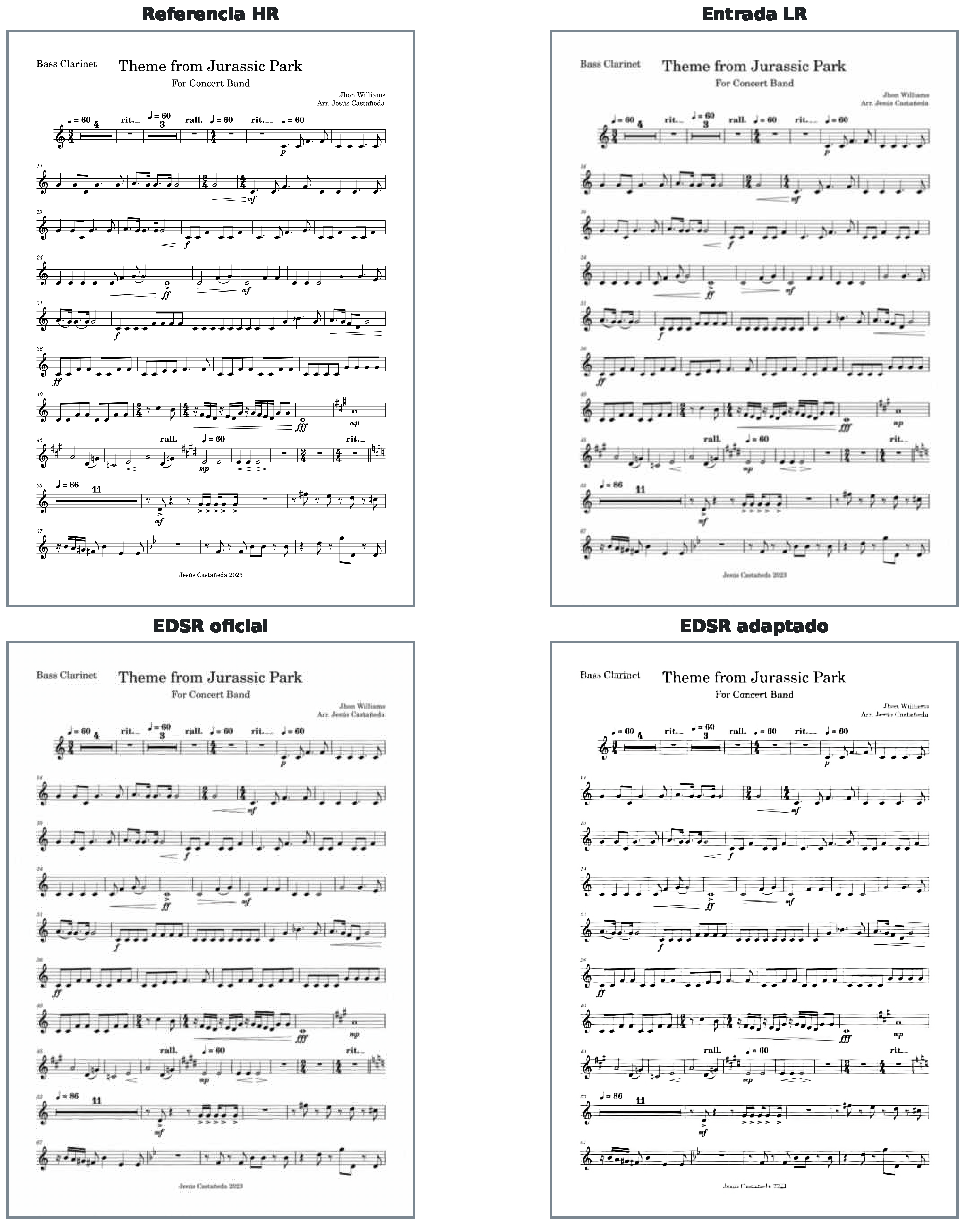
\includegraphics[width=\textwidth,height=0.80\textheight,keepaspectratio]{figures/results/external-jurassic-park-full-page-x4-strong.pdf}
  \caption[Corpus externo: Theme from Jurassic Park, x4 fuerte]{Caso fijo
  \texttt{jurassic-park}, x4 fuerte, aceptado con reservas por daño de LR no recuperado. El EDSR
  adaptado ofrece mayor limpieza que el oficial, pero la degradación fuerte impide recuperar con
  fidelidad texto y símbolos pequeños. Parte de clarinete bajo de \emph{Theme from Jurassic Park},
  música de John Williams. Fuente: archivo musical de la SJMA; página reproducida con autorización
  expresa para este TFG. LR y reconstrucciones son transformaciones de elaboración propia.}
  \label{fig:external-jurassic}
\end{figure}
\clearpage

Las doce páginas deben leerse junto con los recuentos e intervalos del capítulo de resultados. El
atlas hace auditables las decisiones individuales, pero no corrige sus límites: las LR son
sintéticas, hay un único revisor y cada condición contiene solo dos obras. Su valor es mostrar la
heterogeneidad retenida, incluidos los resultados con reservas y el rechazo, no demostrar una tasa
universal de éxito.
